\documentclass[12pt,a4paper]{article}
\usepackage[utf8]{inputenc}
\usepackage[spanish]{babel}
\usepackage{amsmath}
\usepackage{amsfonts}
\usepackage{amssymb}
\usepackage{graphicx}
\usepackage{float}
\usepackage{listings}
\usepackage{xcolor}
\usepackage{hyperref}
\usepackage{booktabs}
\usepackage{array}
\usepackage{longtable}
\usepackage{fancyhdr}
\usepackage{setspace}

% Configuración para reducir espacio en figuras
\setlength{\textfloatsep}{10pt}
\setlength{\floatsep}{10pt}
\setlength{\intextsep}{10pt}

% Configuración de hyperref
\hypersetup{
    colorlinks=true,
    linkcolor=blue,
    filecolor=magenta,      
    urlcolor=cyan,
    citecolor=red
}

% Configuración de listings para código
\lstset{
    basicstyle=\ttfamily\small,
    breaklines=true,
    frame=single,
    numbers=left,
    numberstyle=\tiny,
    keywordstyle=\color{blue},
    commentstyle=\color{green!60!black},
    stringstyle=\color{red},
    backgroundcolor=\color{gray!10}
}

\pagestyle{fancy}
\pagenumbering{arabic}

% Información del documento
\title{\textbf{Desarrollo de un Sistema Modular para el Análisis de Gotas Cargadas Eléctricamente en Tormentas}}
\author{Estudiante de Licenciatura en Ciencias de la Computación}
\date{\today}


\newcommand{\subsubsubsection}[1]{\paragraph{#1}\mbox{}\\}
\setcounter{secnumdepth}{4}
\setcounter{tocdepth}{4}

\begin{document}
\onehalfspacing

\maketitle

\begin{abstract}
    Despues lo hago al abstract
\end{abstract}

\tableofcontents
\newpage

\section{Introducción}
\lhead{}
\rhead{Introducción}

Las gotas de lluvia pueden transportar carga eléctrica, la cual se adquiere principalmente a través de procesos microfísicos dentro de la nube, como las colisiones entre distintos hidrometeoros (granizo, graupel, copos de nieve, cristales de hielo). El signo y la magnitud de estas cargas están estrechamente relacionados las condiciones internas de la tormenta, como la temperatura, el viento, las particular presentes, etc. Al mismo tiempo, la distribución de tamaños de las gotas brinda información sobre la microfísica de la precipitación y resulta esencial para estimar la lluvia, alimentar modelos numéricos, interpretar mediciones de radares y estudiar procesos como la erosión de suelos o crecidas.

En este sentido, medir y analizar simultáneamente el tamaño y la carga de las gotas resulta fundamental, ya que nos permite recopilar información que no solo ayuda a comprender la física de las tormentas, sino que también es útil para mejorar herramientas de pronóstico y para el estudio de fenómenos atmosféricos.

En este marco, ya existen instrumentos capaces de realizar estas mediciones, así como programas para procesarlas. Sin embargo, el código disponible actualmente presenta limitaciones tanto en diseño como en rendimiento: está poco modularizado, resulta difícil de mantener y su desempeño es insuficiente para procesar de manera eficiente grandes volúmenes de datos. En esta tesis se propone un nuevo sistema de análisis que resuelve esas limitaciones, mejorando la eficiencia, la escalabilidad y la mantenibilidad del software, y facilitando así la obtención de resultados más completos y confiables.

\subsection{Instrumento de Medición}
\lhead{}
\rhead{Instrumento de Medición}

El dispositivo utilizado consiste en un anillo de inducción de latón de 6 cm de diámetro y 1.5 cm de longitud, posicionado a 5.7 cm por encima de una placa plana de aluminio de 20 cm de diámetro. Tanto el anillo como la placa están conectados eléctricamente a amplificadores de corriente de alta ganancia con una amplificación de 5 $\times$ 10$^8$ V/A. Para proteger contra interferencias electromagnéticas, el anillo, la placa y los amplificadores están encerrados dentro de un contenedor metálico que actúa como jaula de Faraday. La figura \ref{fig:instrumento_medicion} muestra el dispositivo.

\begin{figure}[!hb]
    \centering
    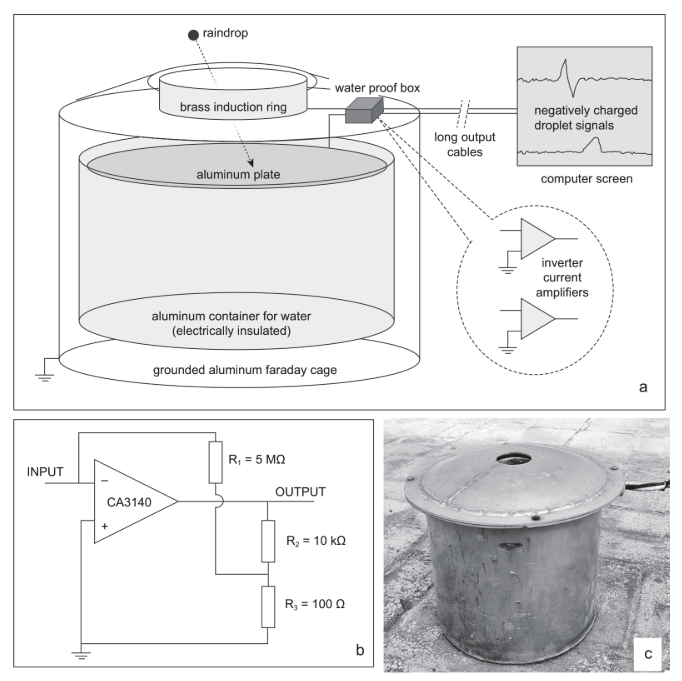
\includegraphics[width=0.7\textwidth]{figures/instrumento_de_medicion.png}
    \caption{(a) Diagrama del dispositivo de medición; (b) circuito amplificador inversor de corriente; (c) fotografía del dispositivo en el techo de la Facultad de Matemática, Astronomía, Física y Computación, Universidad Nacional de Córdoba.}
    \label{fig:instrumento_medicion}
\end{figure}

Los amplificadores están protegidos contra daños por agua al estar asegurados dentro de un recinto impermeable. La jaula de Faraday presenta una abertura ligeramente mayor que el anillo, permitiendo que las gotas de lluvia entren únicamente a través del anillo de inducción. Toda el agua que llega a la placa se drena a través de sus lados y se recolecta en un contenedor de aluminio, que también está situado dentro de la jaula de Faraday pero eléctricamente aislado de ella.

Las gotas cargadas eléctricamente inducen corrientes tanto en el anillo como en la placa. Al caer una gota, primero se acerca al anillo. Al hacerlo, se induce una corriente de la polaridad opuesta a la carga de la gota. Luego, al alejarse, esta polaridad se invierte. Mientras tanto, la gota se acerca a la placa, induciendo también una corriente de polaridad opuesta a la carga de la gota, lo cual culmina en una meseta en la corriente dado que la placa de aluminio absorbe el impacto de la gota y se le transfiere toda la carga a la placa, la cual se disipa en el tiempo. La figura \ref{fig:corriente_gotas} muestra la dinamica de este proceso con el registro de una gota.

\begin{figure}[!hb]
    \centering
    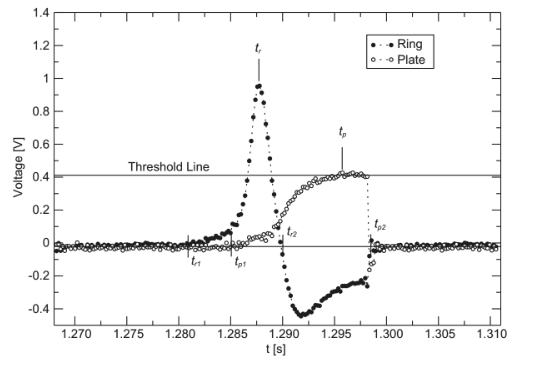
\includegraphics[width=0.7\textwidth]{figures/corriente_gotas.png}
    \caption{Corriente inducida por una gota cargada negativamente en el anillo (puntos solidos) y la placa (puntos huecos).}
    \label{fig:corriente_gotas}
\end{figure}

La adquisición de datos se realiza a una tasa de 5 kHz por canal (5000 datos por segundo). Por limitaciones de hardware, la adquisición de datos no se puede realizar al mismo tiempo que la escritura a disco, por lo que cada segundo se pierden $\sim 50ms$ de datos. Esto debe ser tenido en cuenta luego para analizar los datos obtenidos.

\subsection{Procesamiento de Señales}
\lhead{}
\rhead{Procesamiento de Señales}

El procesamiento transforma las señales crudas registradas por el instrumento en una lista de gotas con sus propiedades. Para ello se emplean dos programas que se ejecutan de manera secuencial: el primero realiza un preprocesamiento de las señales y el segundo extrae las gotas y calcula sus características.
El fragmento de la señal que forma parte de una gota extraida por el programa, la denominamos `pulso`. Estos pulsos son reconocibles en la señal gracias a la dinamica producida por la interaccion de la gota con el instrumento de medicion.
El flujo general consta de cinco pasos principales:

\begin{enumerate}
    \item Rellenado de huecos en los datos.
    \item Remoción del offset de las señales.
    \item Búsqueda de pulsos en las señales.
    \item Aplicación de filtros de calidad para extraer las gotas.
    \item Cálculo de propiedades de las gotas.
\end{enumerate}

Para el procesamiento de los datos se han desarrollado dos programas en Fortran que trabajan de manera secuencial.

El primer programa se encarga del preprocesamiento de los datos, específicamente del rellenado de huecos mediante interpolación lineal y de la remoción del offset de las señales.

El segundo programa realiza el análisis principal de las señales ya preprocesadas. Implementa el algoritmo de detección de pulsos, aplica filtros para separar las gotas válidas y calcula sus propiedades físicas, incluyendo tamaño, carga eléctrica y velocidad de caída.

\subsection{Necesidad de Mejoras}
\lhead{}
\rhead{Necesidad de Mejoras}

El código actual, aunque funcional, sufre de varios problemas tanto en su diseño como en su rendimiento.

En primer lugar, el código consta de pocos archivos con una cantidad de líneas muy grande, lo que dificulta su mantenimiento y modificación. Cualquier cambio requiere revisar y entender todo el código, ya que las responsabilidades no están bien asignadas. Además, hay muchas variables sin nombres descriptivos y constantes hard-codeadas sin referencia alguna, lo que complica aún más la comprensión.

En segundo lugar, para grandes volúmenes de datos, la ejecución es muy lenta. Por ejemplo, para procesar datos de una tormenta de 5 horas de duración (aproximadamente 100M de datos), el programa tarda alrededor de 6 horas en completarse. A esto se suma un consumo de memoria excesivamente alto, lo que obliga a procesar los datos de a partes. A su vez el algoritmo actual no tiene en cuenta las gotas que quedan en medio de estos cortes, resultando en la pérdida de algunos datos.

\subsection{Objetivos}
\lhead{}
\rhead{Objetivos}

\subsubsection{Objetivo General}

Desarrollar un sistema modular y automatizado para el análisis de datos de gotas cargadas eléctricamente que mejore significativamente la eficiencia, mantenibilidad y escalabilidad del código existente, facilitando la obtención de nuevos resultados.

El nuevo sistema debe ser capaz de procesar grandes volúmenes de datos de manera eficiente y, como mínimo, detectar la misma cantidad de gotas que el código original, intentando incrementarla en lo posible.

\subsubsection{Objetivos Específicos}

\begin{enumerate}
    \item \textbf{Diseñar una arquitectura modular} que separe las etapas del procesamiento en al menos tres componentes independientes y reutilizables.

    \item \textbf{Optimizar el rendimiento y el uso de memoria} del algoritmo de detección de gotas para manejar aproximadamente 100 millones de muestras utilizando menos de 2 GB de memoria y reduciendo el tiempo de análisis de una tormenta de 5 horas de 6 horas a aproximadamente 15 minutos, asegurando al menos la misma cantidad de gotas detectadas que el programa original.

    \item \textbf{Desarrollar un sistema de automatización} que permita ejecutar la cadena completa de análisis con un único comando y sin intervención manual.

    \item \textbf{Documentar completamente} el sistema mediante un manual de usuario y comentarios en el código para facilitar su uso y mantenimiento futuro.
\end{enumerate}

\subsection{Estructura de la Tesis}
\lhead{}
\rhead{Estructura de la Tesis}

Despues la hago

\section{Procedimiento}
\lhead{}
\rhead{Procedimiento}

\subsection{Análisis del Código Existente}
\lhead{}
\rhead{Análisis del Código Existente}

Antes de comenzar a desarrollar el nuevo sistema, fue fundamental analizar el código existente. El programa consta de dos archivos Fortran (`promedio\_general.f` y `buscador\_de\_gotas.f`) donde toda la lógica está implementada directamente en el entorno global del programa, sin modularización alguna. 

\subsubsection{Problemas de diseño}

El código existente presenta problemas de diseño que dificultan su comprensión y mantenimiento:

\begin{itemize}

\item \textbf{Modularización inexistente:} Todo el procesamiento está en el entorno global del programa, que maneja todos los pasos de procesamiento, como la detección de pulsos, cálculo de características, aplicación de filtros, escritura de resultados, etc. Cualquier modificación requiere entender por completo como interactuan las diferentes `partes` del programa.

\item \textbf{Variables sin contexto semántico:} El código utiliza variables como `s`, `ss`, `i`,
`j`, `w`, `k`, `l`, `p`, `r`, `x`, `cont`, `contt`, `cc1`, `cc2`, `iii` sin ningún contexto. Es
imposible determinar qué representa cada una sin leer todo el código. Ademas, estan todas definidas en el principio del programa, lo cual hace que sea dificil entender su uso en el resto del código.
    
\item \textbf{Requiere dividir el conjunto de datos en varias partes}: El consumo de memoria es muy alto, por lo que el programa requiere dividir el conjunto de datos en varias partes y procesarlos secuencialmente. Esto hace que se pierdan algunas gotas, ya que las gotas que quedan en medio de los cortes no se procesan.

\item \textbf{Lectura de archivos hard-codeada:} El programa requiere cambio cada vez que se quiera procesar un nuevo conjunto de datos, ya que los nombres de los archivos son constantes en el codigo. Ademas, hay un bloque de codigo que permite leer hasta 36 archivos, que se debe comentar o descomentar dependiendo de la cantidad en la que se dividio el conjunto de datos a procesar.

\item \textbf{Codigo duplicado:} La cantidad de codigo repetido es muy alta. Hay mucha logica la cual solo tiene un cambio en el signo, un cambio en un `if statement` o un cambio en una variable. Esto hace que sea dificil mantener el codigo ya que hay que modificarlo en varios lugares.

\end{itemize}

\subsubsection{Motivación de la refactorización}

Todas las problematicas mencionadas anteriormente, motivan a realizar una refactorizacion del codigo. Esta refactorizacion tiene muchos beneficios, entre los cuales:

\begin{itemize}

\item \textbf{Mantenibilidad:} Cualquier corrección de errores o implementación de mejoras requiere revisar y entender menos codigo, ya que la logica se encuentra en funciones mas pequeñas.

\item \textbf{Reutilizabilidad:} El codigo puede ser reutilizado para otros experimentos o instrumentos.

\item \textbf{Verificación:} Permitiria realizar pruebas unitarias de cada funcion y no de todo el programa completo.

\item \textbf{Colaboración:} Otros investigadores pueden entender y modificar el código sin
invertir tanta cantidad de tiempo y esfuerzo estudiándolo.

\end{itemize}

\subsubsection{Problemas descubiertos durante la refactorización}

El programa `promedio\_general.f`, como se menciono anteriormente, se encarga tanto del rellenado de huecos como de la remocion del offset de las señales. Es en esta primera parte donde se descubrio un error en la implementacion.

Basicamente, primero el algoritmo llena los huecos con un valor constante `10`, para luego buscar los bordes de estos huecos y completarlos con una interpolacion lineal. En los comentarios del codigo, se menciona que esta interpolacion lineal se hace entre los promedios de los 1000 puntos anteriores y posteriores al hueco. Sin embargo, en la implementacion, se utiliza los valores de los extremos del huecos.

El código \ref{lst:codigo_error} muestra la implementación del algoritmo de rellenado de huecos. Como se puede observar, los comentarios indican que se debe usar el promedio de 1000 puntos, pero la implementación utiliza directamente los valores de los bordes (`a1`, `a2`, `b1`, `b2`).

Este error tiene un impacto significativo en los pasos posteriores del procesamiento, particularmente en la remoción del offset. Al rellenar los huecos utilizando una interpolación entre dos valores puntuales, en lugar de promedios de ventanas más amplias, se pueden introducir distorsiones importantes. Esto ocurre especialmente cuando los valores utilizados para la interpolación corresponden a puntos críticos que difieren considerablemente del promedio de la señal en ese momento.

\begin{lstlisting}[language=Fortran, label=lst:codigo_error]
* Busca donde esta un punto que tiene valor de 10. y 
* va hacia atras para encontrar el primer que no es
* igual a 10.
* es decir es un borde izquierdo de un 'hueco'
* tambien va hacia adelante para encontrar el borde
* derecho del 'hueco'
* despues promedia los numeros de cada canal
* 100 puntos hacia atras
* y 1000 puntos hacia adelante 
* y a esos promedios los llama a1 y a2 para el 
* primer canal y
* b1 y b2 para el segundo canal
* Despues el valor w1(j) y w2(j) los revalua como
* siguiendo una recta 
* entre esos dos promedios.
* Tambien ingresa un indice que vale 1 cunado no hay
* blanco y un 0 cuando si lo hay.

      do j=1,ww
         if (w1(j).eq.10.) then
            ind(j)=0
            
            do i=1,ww
               if ((j-i.gt.0.).and.(w1(j-i).ne.10.)) then
		     a1=w1(j-i)
		     b1=w2(j-i)                  
                     k1=i
                  goto 20
               endif
            enddo
            
 20         do i=1,ww  
               if ((j+i.le.ww).and.(w1(j+i).ne.10.)) then
		     a2=w1(j+i)
		     b2=w2(j+i)                  
                     k2=i-1
                  goto 30
               endif
            enddo

! Aca es donde se utiliza los valores de los extremos
! en vez de los promedios de 1000 puntos
 30         w1p(j)=(a2-a1)/real(k2+k1)*real(k1)+a1
            w2p(j)=(b2-b1)/real(k2+k1)*real(k1)+b1
         else
            ind(j)=1
            w1p(j)=w1(j)
            w2p(j)=w2(j)
         endif
      enddo
\end{lstlisting}


\subsubsection{Descripción del algoritmo actual}
Como se menciono anteriormente, el sistema de procesamiento actual consta de dos programas que se ejecutan
secuencialmente.

\subsubsubsection{Programa de preprocesamiento}

El primer programa (`promedio\_general.f`) recibe como entrada las señales crudas registradas por el instrumento y realiza dos operaciones fundamentales:    

\begin{enumerate}
    \item \textbf{Rellenado de huecos mediante interpolación:} Debido a las limitaciones de
hardware mencionadas anteriormente, cada segundo se pierden aproximadamente
$50ms$ de datos durante la adquisición. El programa identifica estos huecos y los
rellena utilizando interpolación lineal entre los puntos adyacentes.

\textbf{Nota importante:} Esta es la parte del programa que fue modificada para corregir el error en la implementación del rellenado de huecos.

\item \textbf{Remoción del offset de las señales:} Para cada punto de la señal, se calcula el
promedio de los 5000 puntos circundantes (2500 puntos a cada lado) y se resta este
valor al punto central. Este proceso elimina el offset de corriente continua que puede
variar durante la medición.

\textbf{Nota importante:} Como a cada punto se le resta el promedio de los 5000 puntos circundantes, los valores que se encuentran cercanos a los huecos, se ven afectados por el error en la implementación del paso anterior. Como el valor del offset puede cambiar entre los 2 extremos de un hueco, el promedio calculado se aleja del valor real, haciendo que estos puntos no se les pueda eliminar completamente el offset.

\end{enumerate}

La salida de este programa son las señales preprocesadas: sin huecos y con el offset
removido, listas para ser analizadas por el segundo programa.

\subsubsubsection{Programa de detección de gotas}

El segundo programa (`buscador\_de\_gotas.f`) implementa el algoritmo principal de
detección y análisis. El flujo general consta de las siguientes etapas:

\begin{enumerate}

\item \textbf{Lectura y preprocesamiento de datos:} El programa lee los archivos de datos
preprocesados que contienen las señales del anillo y la placa. Se pueden leer hasta
36 archivos, y cada archivo puede contener hasta 13 millones de muestras.

\item \textbf{Detección de pulsos mediante umbrales:} Se implementa un sistema de umbrales que varía dinámicamente desde un valor superior (`c1=2.00`) hasta
uno inferior (`c2=0.02`) a lo largo de 1000 pasos (`ps=1000`). Esta variación permite
detectar pulsos de diferentes amplitudes.
Para cada umbral, se buscan pares de puntos consecutivos que superen el umbral en ambas señales (anillo y placa), con una separación máxima de 100 puntos
(`nn=100`).

\item \textbf{Localización y delimitación de pulsos:} Una vez detectado un pulso, se determina su inicio retrocediendo hasta encontrar el punto donde la señal se anula. Se
calcula el punto medio del primer pulso (anillo) y el punto de quiebre del segundo
pulso (placa) mediante análisis de la integral de la señal.
El algoritmo recorta cada pulso considerando un ancho máximo de $4\times nn$ puntos,
adaptándose dinámicamente según la duración real del evento.

\item \textbf{Cálculo de propiedades físicas:} Para cada pulso detectado, se calculan:

\begin{itemize}
    \item Carga eléctrica: Se integra la señal de ambos canales y se aplica el factor de
    conversión correspondiente a la amplificación del instrumento.
    \item Velocidad de caída: Se determina mediante la separación conocida entre
    anillo y placa (5.7 cm) dividida por el tiempo entre picos de la señal.
    \item Diámetro: Se obtiene interpolando en una tabla velocidad-diámetro precalculada.
\end{itemize}

\item \textbf{Aplicación de filtros de calidad:} Se implementan filtros secuenciales para separar
las gotas válidas del ruido:

\begin{itemize}

\item \textbf{Filtros de carga:} La carga de la gota tanto en el anillo como en la placa tiene
que ser mayor a un valor mínimo (`qminima=0.2`) (en valor absoluto).

\item \textbf{Filtro de velocidad:} Se verifica que la distancia temporal entre los picos del
anillo y la placa corresponda a una velocidad de caída físicamente plausible
(entre 0.7125 y 11.4 m/s).

\item \textbf{Filtro de signo:} Se verifica que la carga de la gota sea del mismo signo en
ambos canales.
\end{itemize}

\item \textbf{Sistema de penalización y ordenamiento:} Se implementa un sistema de puntuación que evalúa la calidad de cada detección mediante cinco criterios:

\begin{itemize}

    \item \textbf{Penal1 y Penal2:} Diferencia cuadrática entre la señal real y 2 modelos teóricos distintos
    del pulso.
    \item \textbf{Penal3:} Desviación de la proporción esperada entre cargas del anillo y la placa.
    \item \textbf{Penal4:} Desviación de la proporción esperada del ancho entre los picos de la
señal de la placa y el anillo.
    \item \textbf{Penal5:} Proporción de señal en el rango de ruido (entre -0.02 y 0.02).
\end{itemize}
    La suma de estas penalizaciones determina el orden de calidad de las gotas detectadas, permitiendo filtrar los resultados según la precisión requerida.

\item \textbf{Salida de resultados:} Finalmente, se escriben los datos de todas las gotas válidas
en un archivo, incluyendo posición temporal, cargas, velocidad, diámetro y puntuación de calidad.


\end{enumerate}

\subsection{Algoritmos y estructuras de datos utilizadas}
\lhead{}
\rhead{Algoritmos y estructuras de datos utilizadas}

Para abordar las limitaciones del código existente, se utilizaron algoritmos y estructuras de datos eficientes que mantienen la misma o similar funcionalidad pero con un
rendimiento mejor.

\subsubsection{Optimización del algoritmo de promedio móvil}

El código Fortran original implementaba la remoción de offset mediante un promedio
móvil de 5000 puntos de manera ineficiente. Para cada punto, se calculaba la suma de 5000
valores y se realizaba una división en cada uno de estos, resultando en una complejidad
$O(5000n) = O(n)$ pero con una constante extremadamente alta.

\textbf{Implementación original (ineficiente):} El algoritmo original realizaba las siguientes
operaciones para cada punto:

Esta implementación presenta varios problemas:

\begin{itemize}
    \item \textbf{Complejidad:} $O(5000n)$ operaciones, donde la constante 5000 es extremadamente alta
    \item \textbf{Operaciones repetitivas:} Cada punto recalcula la suma completa de la ventana
    \item \textbf{Uso de memoria:} No aprovecha la superposición entre ventanas consecutivas
    \item \textbf{Divisones múltiples:} 5000 divisiones por cada punto procesado
\end{itemize}

\textbf{Implementación optimizada:} El nuevo algoritmo implementa un promedio móvil eficiente que mantiene la misma funcionalidad pero con una complejidad constante mucho
menor:

\textbf{Análisis de complejidad:} La implementación optimizada mantiene la misma complejidad $O(n)$ pero con una constante dramáticamente reducida:

\begin{itemize}
    \item \textbf{Operaciones por punto:} Solo 1 suma, 1 resta y 1 división (cuando la ventana está
    completa)
    \item \textbf{Complejidad total:} $O(n)$ con constante cercana a 3
    \item \textbf{Mejora en constante:} De 5000 a 3, una reducción de más de 1600 veces
\end{itemize}

\subsubsection{Estructura de datos MaxMinQueue}

Para la detección eficiente de pulsos en las señales, se implementó una estructura de
datos especializada que permite obtener el máximo y mínimo de una ventana deslizante
en tiempo constante $O(1)$.

\textbf{Problema a resolver:} El algoritmo original de detección de pulsos requería encontrar
el máximo y mínimo en ventanas de diferentes tamaños para cada punto de la señal. Una
implementación ingenua tendría complejidad $O(w)$ por ventana, donde w es el tamaño de
la ventana, resultando en una complejidad total de $O(n \times w)$.

\textbf{Implementación de MaxMinQueue:} La estructura utiliza dos deques (double-ended
queues) para mantener los máximos y mínimos de manera eficiente:

\textbf{Operación de inserción (push):} La inserción mantiene los deques ordenados para
garantizar acceso $O(1)$ a máximo y mínimo:

\textbf{Operación de extracción (pop):} La extracción actualiza los deques de máximo y
mínimo cuando se remueve el elemento correspondiente:

\textbf{Acceso a máximo y mínimo:} Las operaciones de acceso son constantes $O(1)$:

\textbf{Análisis de complejidad:}

\begin{itemize}
    \item \textbf{Inserción (push):} $O(1)$ amortizado - aunque en el peor caso puede ser $O(w)$, la
amortización garantiza $O(1)$ por operación
    \item \textbf{Extracción (pop):} $O(1)$ - solo actualiza contadores y posiblemente remueve un
    elemento del deque
    \item \textbf{Acceso a máximo/minimo:} $O(1)$ - siempre accede al primer elemento del deque
    correspondiente
    \item \textbf{Memoria:} $O(w)$ donde w es el tamaño de la ventana
\end{itemize}

\textbf{Aplicación en detección de pulsos:} La MaxMinQueue se utiliza para implementar
ventanas deslizantes eficientes en la detección de pulsos:

\textbf{Ventajas sobre implementaciónes tradicionales:}

\begin{itemize}
    \item \textbf{Rendimiento:} Acceso $O(1)$ a máximo y mínimo en lugar de $O(w)$
    \item \textbf{Escalabilidad:} El rendimiento no se degrada con el tamaño de la ventana
    \item \textbf{Flexibilidad:} Permite implementar diferentes estrategias de detección
    \item \textbf{Reutilizabilidad:} Estructura genérica que puede aplicarse a otros problemas
\end{itemize}

\subsection{Implementación en C++}
\lhead{}
\rhead{Implementación en C++}

Toda la explicacion del codigo de C++

\subsection{Sistema de Automatización}
\lhead{}
\rhead{Sistema de Automatización}

Toda la explicacion del codigo de Python

\section{Resultados}

- Comparativas de tiempo
- Comparativas de memoria
- Comparativas de cantidad de gotas detectadas

Señalar todos los objetivos cumplidos en base a los planteados

\subsection{Limitaciones y Áreas de Mejora}
\lhead{}
\rhead{Limitaciones y Áreas de Mejora}

Despues vemos

\section{Conclusiones}

Veremos 

\section{Referencias}

\begin{enumerate}
    \item Despues las hago
\end{enumerate}

\end{document}
